\documentclass[11pt]{beamer}
\usepackage[utf8]{inputenc}
\usepackage{graphicx, epsfig}
\usepackage{amsmath,mathrsfs,amsfonts,amssymb}
%\usepackage{subfig}
\usepackage{floatflt}
\usepackage{epic,ecltree}
\usepackage{mathtext}
\usepackage{fancybox}
\usepackage{fancyhdr}
\usepackage{multirow}
\usepackage{enumerate}
\usepackage{epstopdf}
\usepackage{multicol}
\usepackage{algorithm}
\usepackage[noend]{algorithmic}
\usepackage{tikz}
\usepackage{blindtext}
\usetheme{default}%{default}%{Singapore}%{Warsaw}%{Warsaw}%{Darmstadt}
\usecolortheme{default}
\setbeamerfont{title}{size=\Huge}
\setbeamertemplate{footline}[page number]{}


\makeatletter
\newcommand\HUGE{\@setfontsize\Huge{35}{40}}
\makeatother    

\setbeamerfont{title}{size=\HUGE}
\beamertemplatenavigationsymbolsempty

% latin bold lower
\newcommand{\ba}{\mathbf{a}} 
\newcommand{\bc}{\mathbf{c}} 
\newcommand{\be}{\mathbf{e}} 
\newcommand{\bh}{\mathbf{h}} 
\newcommand{\bp}{\mathbf{p}} 
\newcommand{\bt}{\mathbf{t}} 
\newcommand{\bs}{\mathbf{s}} 
\newcommand{\bu}{\mathbf{u}} 
\newcommand{\bv}{\mathbf{v}} 
\newcommand{\bw}{\mathbf{w}} 
\newcommand{\bx}{\mathbf{x}} 
\newcommand{\by}{\mathbf{y}} 
\newcommand{\bz}{\mathbf{z}} 

% latin bold upper
\newcommand{\bA}{\mathbf{A}} 
\newcommand{\bB}{\mathbf{B}} 
\newcommand{\bC}{\mathbf{C}} 
\newcommand{\bI}{\mathbf{I}} 
\newcommand{\bL}{\mathbf{L}} 
\newcommand{\bM}{\mathbf{M}} 
\newcommand{\bQ}{\mathbf{Q}} 
\newcommand{\bT}{\mathbf{T}} 
\newcommand{\bU}{\mathbf{U}} 
\newcommand{\bV}{\mathbf{V}} 
\newcommand{\bW}{\mathbf{W}} 
\newcommand{\bX}{\mathbf{X}} 
\newcommand{\bY}{\mathbf{Y}} 
\newcommand{\bZ}{\mathbf{Z}} 

% latin cal upper
\newcommand{\cG}{\mathcal{G}} 
\newcommand{\cL}{\mathcal{L}} 
\newcommand{\cN}{\mathcal{N}} 
\newcommand{\cS}{\mathcal{S}} 
\newcommand{\cT}{\mathcal{T}} 
\newcommand{\cW}{\mathcal{W}} 
\newcommand{\cX}{\mathcal{X}} 
\newcommand{\cZ}{\mathcal{Z}} 

% latin bb upper
\newcommand{\bbE}{\mathbb{E}} 
\newcommand{\bbI}{\mathbb{I}} 
\newcommand{\bbP}{\mathbb{P}} 
\newcommand{\bbR}{\mathbb{R}} 

% greek bold lower
\newcommand{\bepsilon}{\boldsymbol{\epsilon}} 
\newcommand{\btheta}{\boldsymbol{\theta}} 
\newcommand{\blambda}{\boldsymbol{\lambda}} 
\newcommand{\bpi}{\boldsymbol{\pi}} 
\newcommand{\bmu}{\boldsymbol{\mu}} 
\newcommand{\bsigma}{\boldsymbol{\sigma}} 
\newcommand{\bphi}{\boldsymbol{\phi}} 

% greek bold upper
\newcommand{\bSigma}{\boldsymbol{\Sigma}} 

\DeclareMathOperator*{\argmin}{arg\,min}
\DeclareMathOperator*{\argmax}{arg\,max}
\newcommand{\createdgmtitle}[1]{\title[\hbox to 56mm{Mathematical Forecasting Methods \hfill\insertframenumber\,/\,\inserttotalframenumber}]
	{\vspace{1.5\cm} \\ Mathematical Forecasting Methods \\ {\Huge Лекция #1}}
	\author{}
	\institute{
	МФТИ
	} 
	\date{Осень, 2023}
}

\newcommand\myfootnote[1]{%
  \tikz[remember picture,overlay]
  \draw (current page.south west) +(1in + \oddsidemargin,0.5em)
  node[anchor=south west,inner sep=0pt]{\parbox{\textwidth}{%
      \rlap{\rule{10em}{0.4pt}}\raggedright\scriptsize \textit{#1}}};}

\newcommand\myfootnotewithlink[2]{%
  \tikz[remember picture,overlay]
  \draw (current page.south west) +(1in + \oddsidemargin,0.5em)
  node[anchor=south west,inner sep=0pt]{\parbox{\textwidth}{%
      \rlap{\rule{10em}{0.4pt}}\raggedright\scriptsize\href{#1}{\textit{#2}}}};}
\createdgmtitle{1}
\usepackage{tikz}
\usepackage[english,russian]{babel}
\usetikzlibrary{arrows,shapes,positioning,shadows,trees}



%--------------------------------------------------------------------------------
\begin{document}
%--------------------------------------------------------------------------------
\begin{frame}[noframenumbering,plain]
%\thispagestyle{empty}
\titlepage
\end{frame}
%=======
\begin{frame}{Forecasting Methods/Models zoo}
    \begin{figure}
        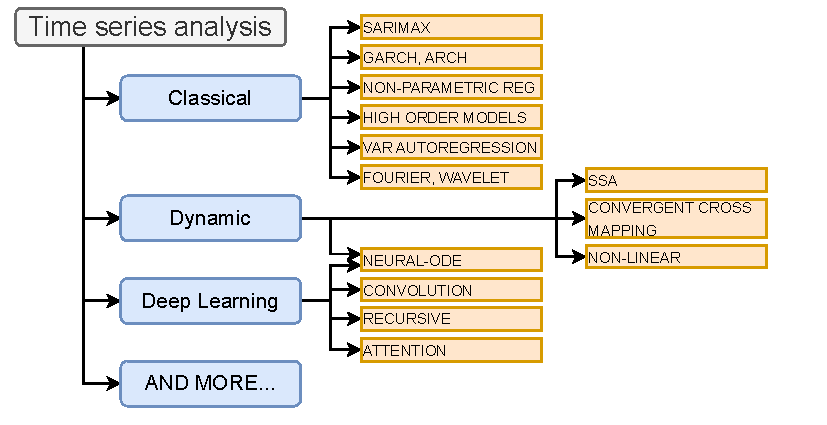
\includegraphics[width=1.1\linewidth, left]{./figs/init_diagram.pdf}
    \end{figure}
\end{frame}
%=======
\begin{frame}{Регрессионные модели: непараметрические методы}
	\begin{figure}
		\centering
		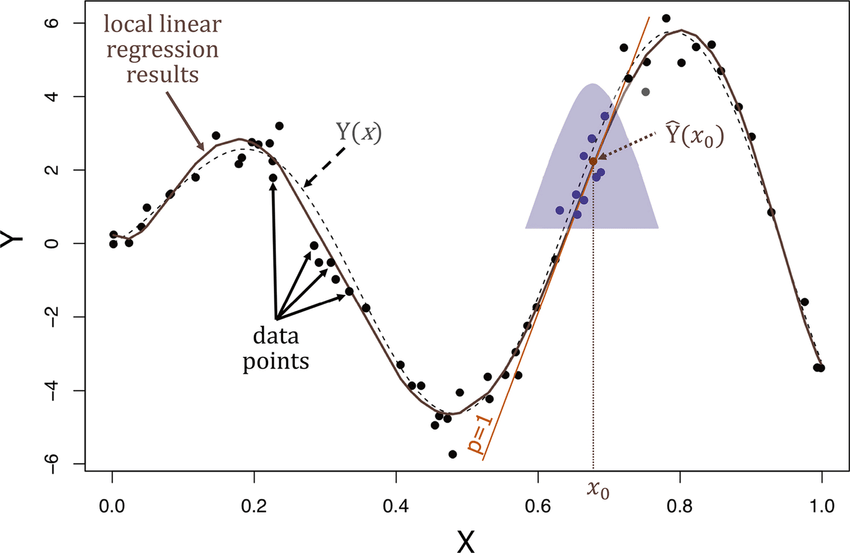
\includegraphics[width=0.8\linewidth]{lecture_1/figs/kernel_reg.png}
	\end{figure}
	\myfootnotewithlink{https://jcheminf.biomedcentral.com/articles/10.1186/s13321-021-00484-5}{сredit: https://jcheminf.biomedcentral.com/articles/10.1186/s13321-021-00484-5}
\end{frame}
%=======
\begin{frame}{Регрессионные модели: автокорреляция}
	\begin{figure}
		\centering
		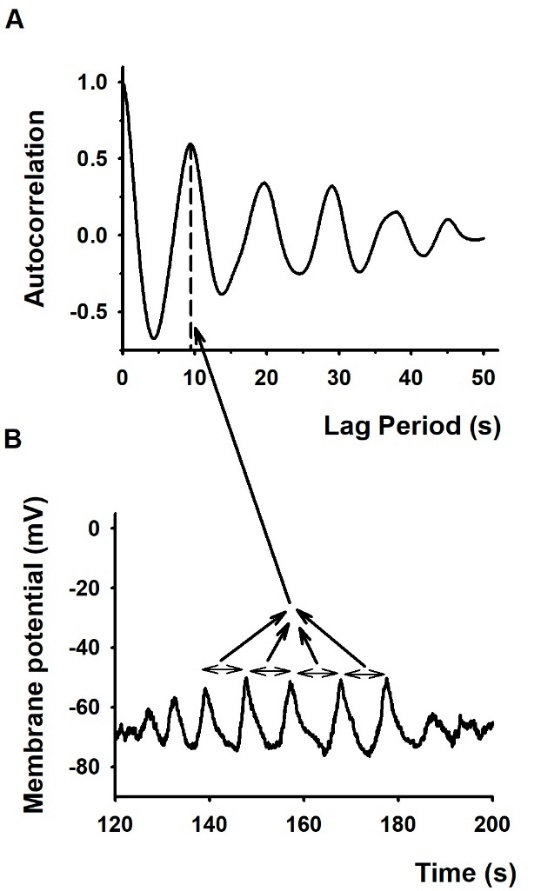
\includegraphics[width=0.4\linewidth]{lecture_1/figs/autocorr.png}
	\end{figure}
	\myfootnotewithlink{https://www.researchgate.net/publication/345125392_Data-Driven_Anomaly_Detection_Approach_for_Time-Series_Streaming_Data?_tp=eyJjb250ZXh0Ijp7ImZpcnN0UGFnZSI6Il9kaXJlY3QiLCJwYWdlIjoiX2RpcmVjdCJ9fQ}{сredit: https://www.researchgate.net/publication/345125392_Data-Driven_Anomaly_Detection_Approach_for_Time-Series_Streaming_Data}
\end{frame}
%=======
\begin{frame}{Регрессионные модели: SARIMAX}
	\begin{figure}
		\centering
		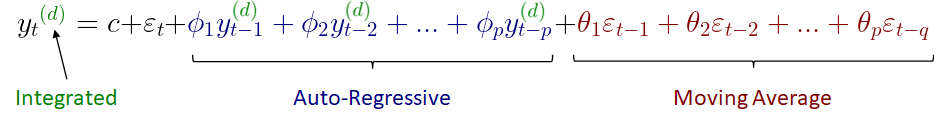
\includegraphics[width=0.8\linewidth]{lecture_1/figs/arima_1.png}
        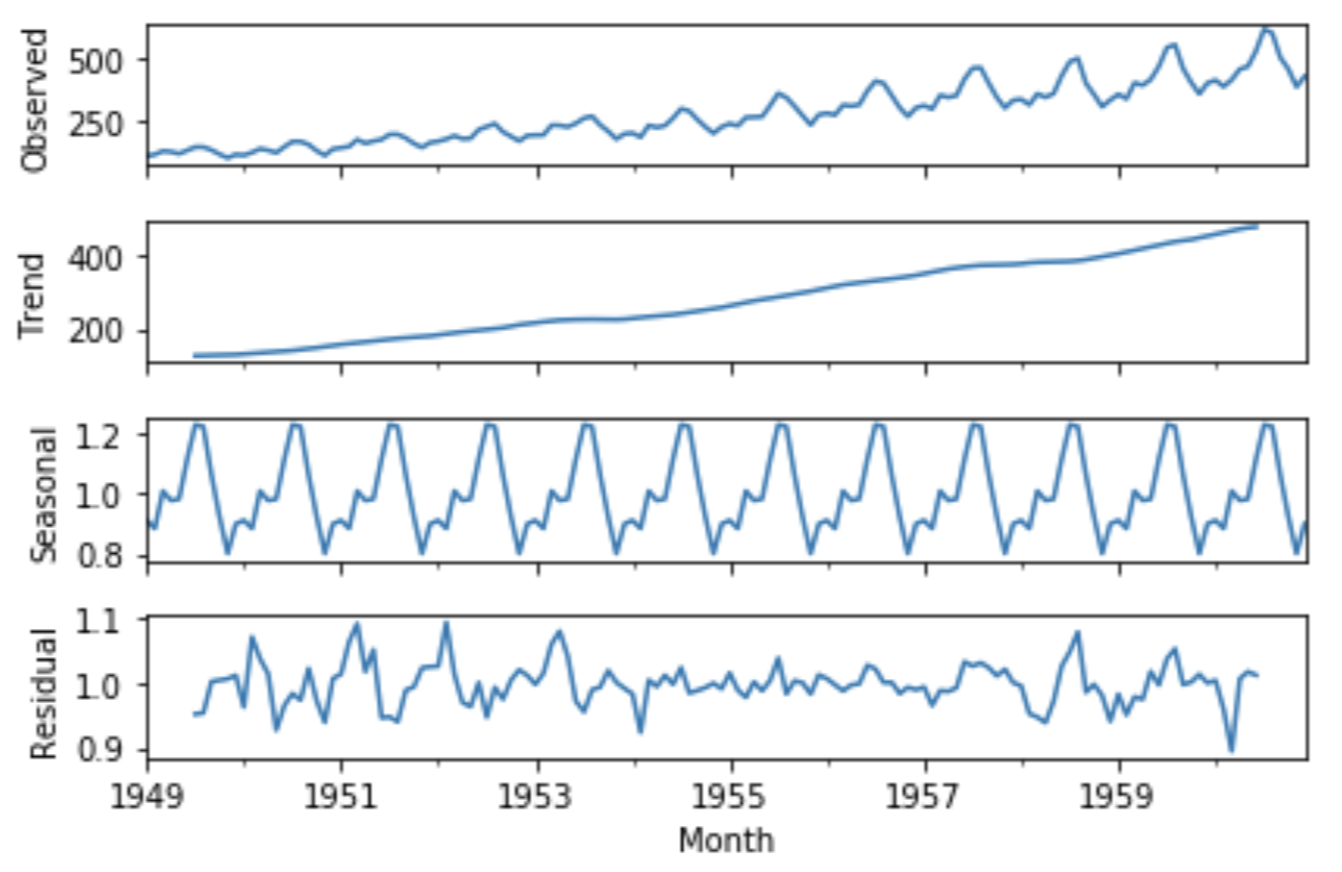
\includegraphics[width=0.7\linewidth]{lecture_1/figs/arima_2.png}
	\end{figure}
	\myfootnotewithlink{https://www.geeksforgeeks.org/python-arima-model-for-time-series-forecasting/}{сredit: https://www.geeksforgeeks.org/python-arima-model-for-time-series-forecasting/}
\end{frame}
%=======
\begin{frame}{Регрессионные модели: сверточные нейронные сети}
	\begin{figure}
		\centering
		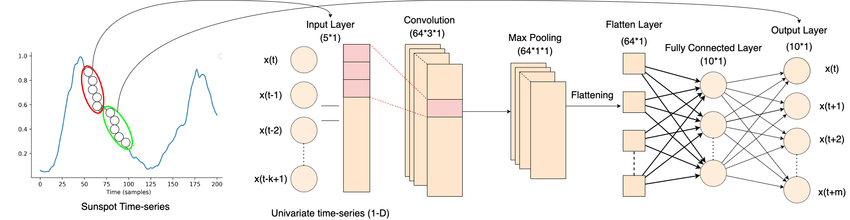
\includegraphics[width=\linewidth]{lecture_1/figs/One-dimensional-Convolutional-Neural-Network-for-time-series.png}
	\end{figure}
	\myfootnotewithlink{https://jmtomczak.github.io/blog/1/1\_introduction.html}{сredit: https://jmtomczak.github.io/blog/1/1\_introduction.html}
\end{frame}
%=======
\begin{frame}{Регрессионные модели: рекуррентные нейронные сети}
	\begin{figure}
		\centering
		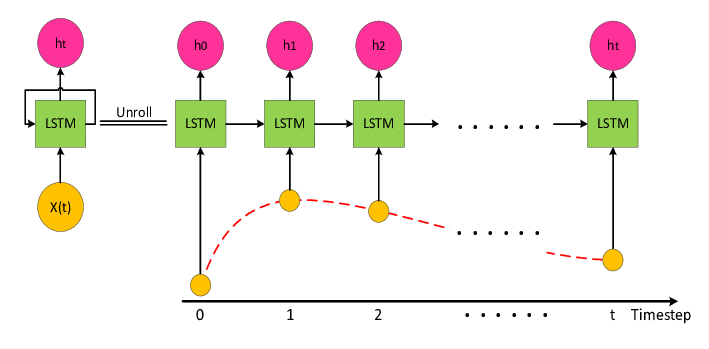
\includegraphics[width=\linewidth]{lecture_1/figs/lstm.png}
	\end{figure}
	\myfootnotewithlink{https://ieeexplore.ieee.org/document/8736879}{сredit: https://ieeexplore.ieee.org/document/8736879}
\end{frame}
%=======
\begin{frame}{От статистическких к динамическим}
	\begin{figure}
		\centering
		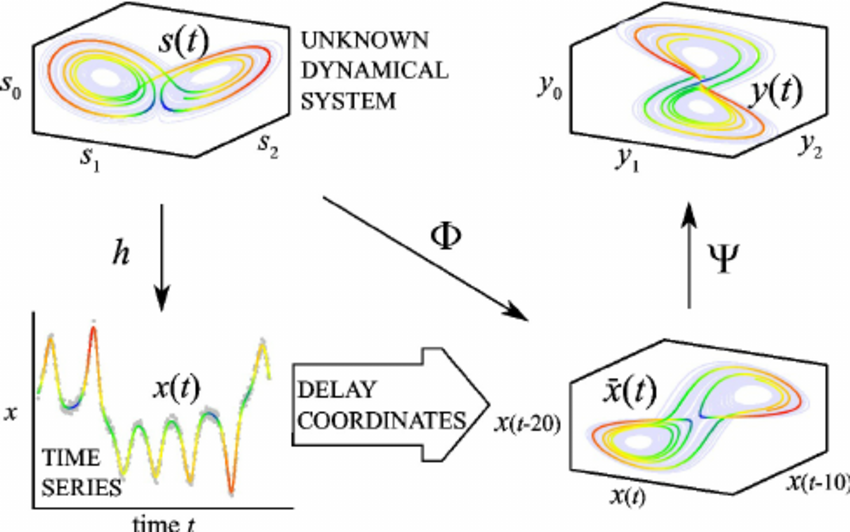
\includegraphics[width=0.8\linewidth]{lecture_1/figs/takens.png}
	\end{figure}
	\myfootnotewithlink{https://phdinds-aim.github.io/time_series_handbook/06_ConvergentCrossMappingandSugiharaCausality/ccm_sugihara.html}{сredit: https://phdinds-aim.github.io/time_series_handbook/06_ConvergentCrossMappingandSugiharaCausality/ccm_sugihara.html}
\end{frame}
%=======
\begin{frame}{От статистическких к динамическим: перекретсное отображение}
	\begin{figure}
		\centering
		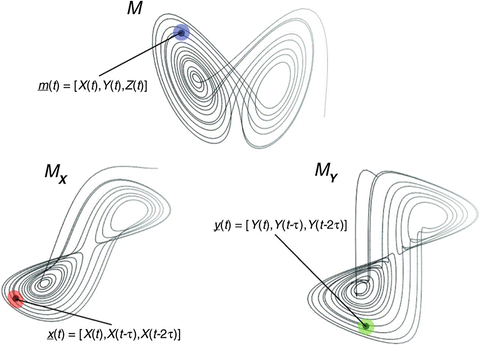
\includegraphics[width=0.7\linewidth]{lecture_1/figs/ssm.png}
	\end{figure}
	\myfootnotewithlink{https://phdinds-aim.github.io/time_series_handbook/06_ConvergentCrossMappingandSugiharaCausality/ccm_sugihara.html}{сredit: https://phdinds-aim.github.io/time_series_handbook/06_ConvergentCrossMappingandSugiharaCausality/ccm_sugihara.html}
\end{frame}
%=======
\begin{frame}{От статистическких к динамическим: фурье анализ}
	\begin{figure}
		\centering
		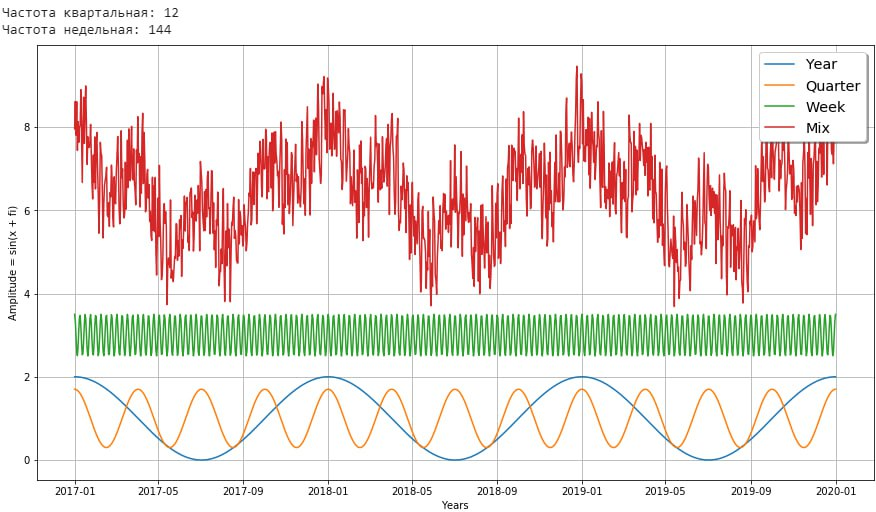
\includegraphics[width=1\linewidth]{lecture_1/figs/fourier.jpg}
	\end{figure}
	\myfootnotewithlink{https://www.bizkit.ru/2020/01/21/16486/}{сredit: https://www.bizkit.ru/2020/01/21/16486/}
\end{frame}
%=======
\begin{frame}{От статистическких к динамическим: вейвлет преобразование}
	\begin{figure}
		\centering
		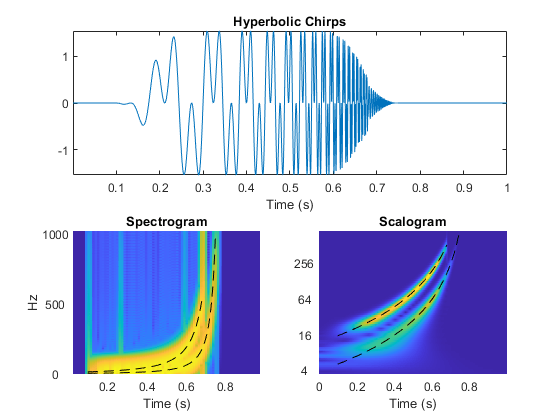
\includegraphics[width=0.8\linewidth]{lecture_1/figs/wavelet.png}
	\end{figure}
	\myfootnotewithlink{https://www.mathworks.com/help/wavelet/gs/choose-a-wavelet.html}{сredit: https://www.mathworks.com/help/wavelet/gs/choose-a-wavelet.html}
\end{frame}
%=======
\begin{frame}{От статистическких к динамическим: сингулярный спектральный анализ}
	\begin{figure}
		\centering
		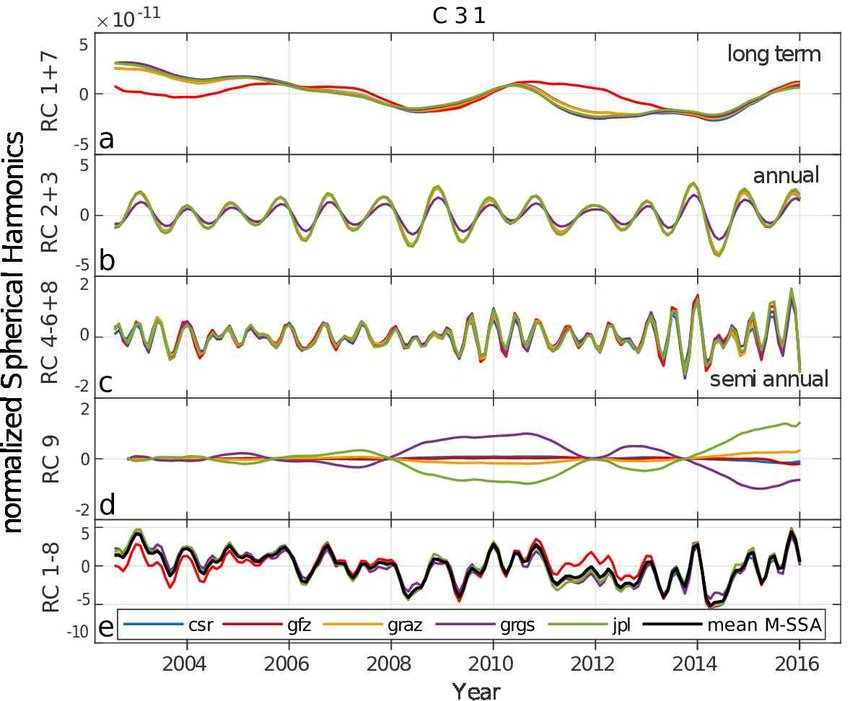
\includegraphics[width=0.8\linewidth]{./figs/ssa.jpg}
	\end{figure}
	\myfootnotewithlink{http://dx.doi.org/10.1093/gji/ggz409}{сredit: http://dx.doi.org/10.1093/gji/ggz409}
\end{frame}
%=======
\begin{frame}{Тензорные методы}
	\begin{figure}
		\centering
		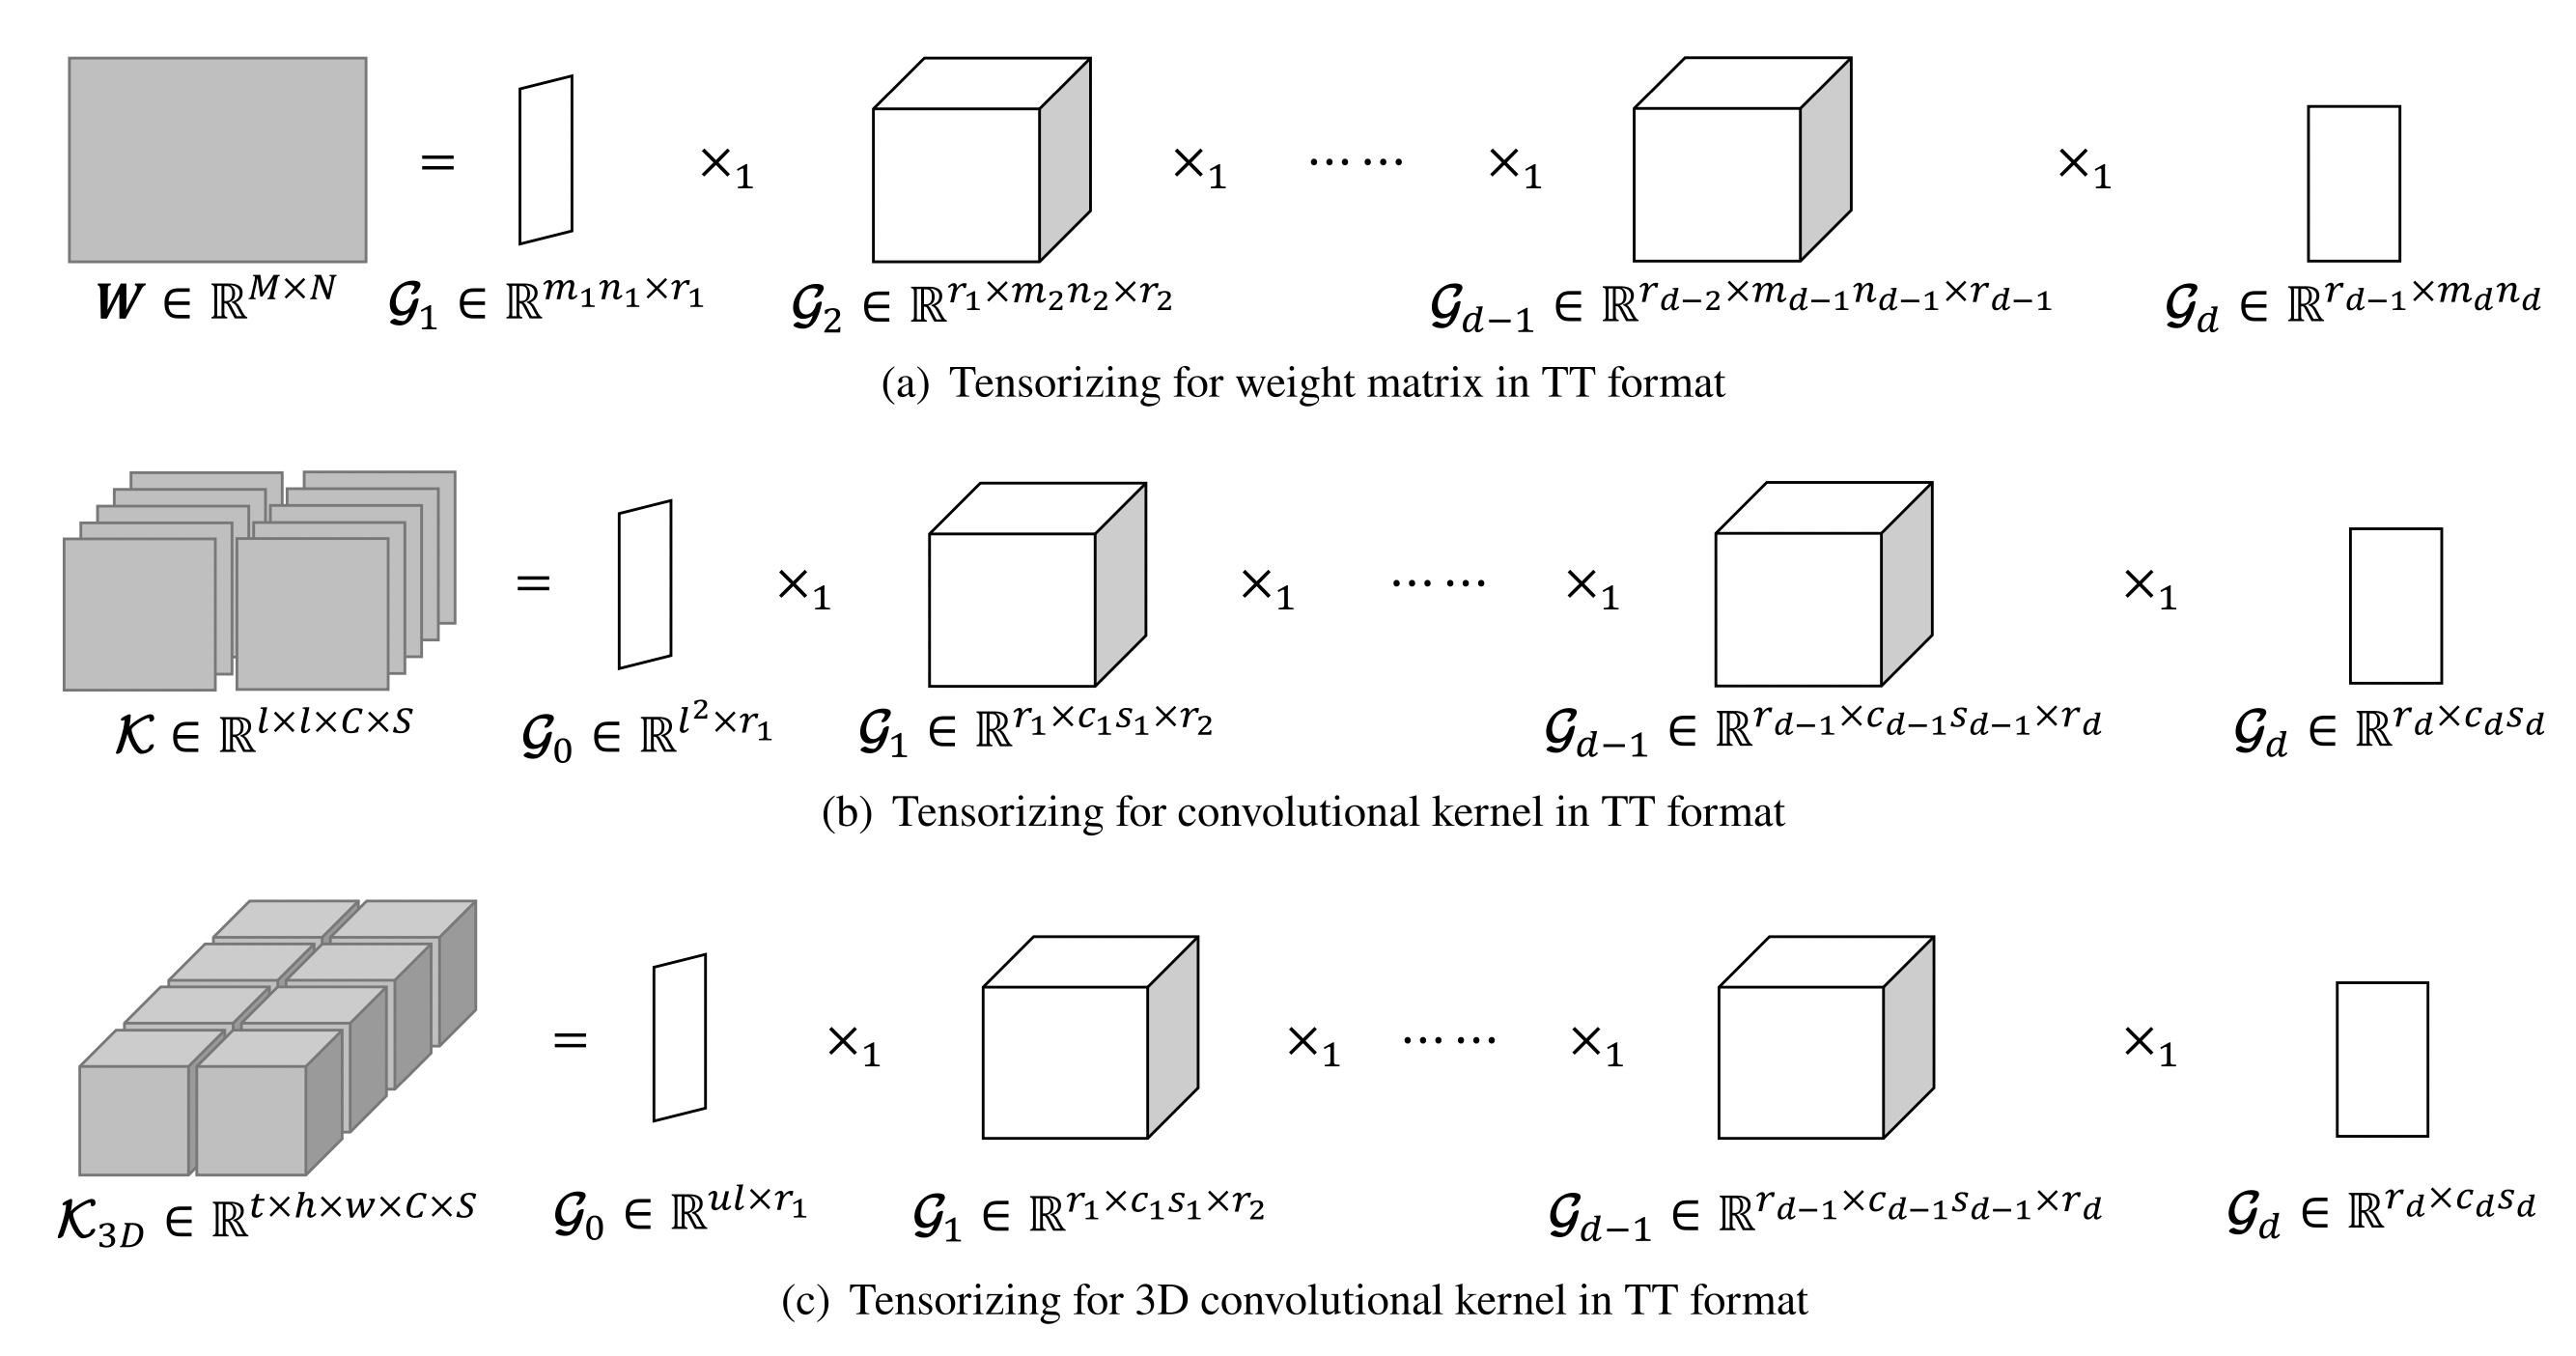
\includegraphics[width=\linewidth]{./figs/tensor_train.png}
	\end{figure}
	\myfootnotewithlink{https://doi.org/10.1016/j.neunet.2020.07.028}{сredit: https://doi.org/10.1016/j.neunet.2020.07.028}
\end{frame}
%=======
\begin{frame}{Дифференциальные модели: Neural-ODE}
	\begin{figure}
		\centering
		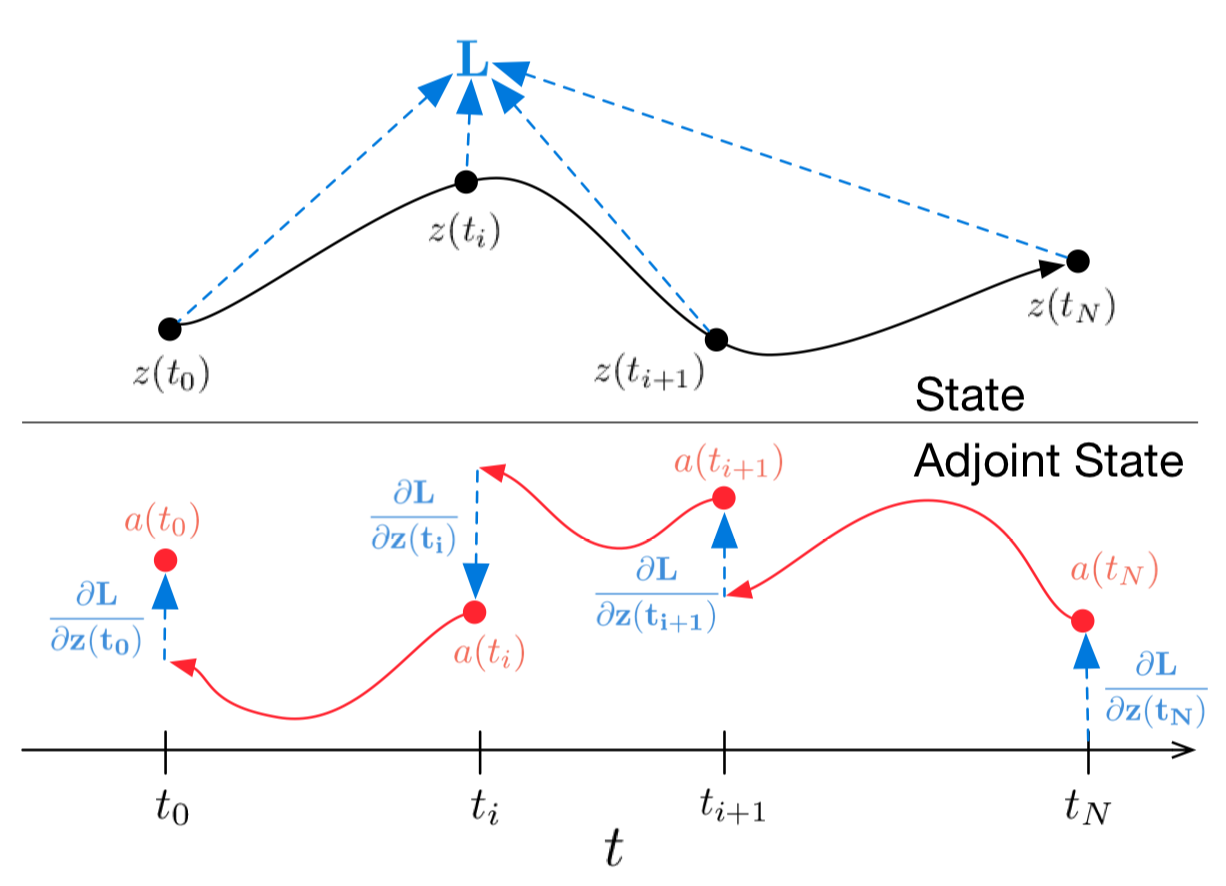
\includegraphics[width=0.9\linewidth]{lecture_1/figs/neuralode.png}
	\end{figure}
	\myfootnotewithlink{https://habr.com/ru/companies/ods/articles/442002/}{сredit: https://habr.com/ru/companies/ods/articles/442002/}
\end{frame}
%=======
\begin{frame}{Временноя ряд}
\begin{itemize}
    \item Временным рядом --- это последовательность значений некоторой переменной (или переменных), регистрируемых непрерывно или через некоторые промежутки времени.
    
    \item Скалярным временным рядом $\{x_i\}_{i=1}^{N}$ называется массив из N чисел, представляющих собой значения некоторой измеренной (наблюдаемой) динамической переменной $x(t)$ с некоторым постоянным шагом $\tau$ по времени, $t_i = t_0 + (i - 1)\tau : x_i = x(t_i), i = 1,..., N$.

    \item Основные задачи --- это задача прогноза (предсказать будущие значения измеряемых характеристик изучаемого объекта на некоторый отрезок времени вперед).
\end{itemize}
\end{frame}
%=======
\begin{frame}{Временноя ряд}
$\{x_t\}_{t=1}^{N}$ --- временным рядом,

$\hat{x}_{t+d} = f_{t,d}(x_1,...x_N;w)$ --- модель временного ряда, где $d =1,...,D$ --- горизонт прогнозирования,

Метод наименьших квадратов:
    \begin{equation*}
        Q_t(w) = \sum_{i = t_0}^{t}(\hat{x}_{i}(w) - x_i)^2 \rightarrow \min_w
    \end{equation*}

Проблемы:
\begin{itemize}
    \item может быть сложная структура временных рядов,
    \item неквадратичная функция потерь,
    \item учитывать физическую природу временного ряда.
\end{itemize}
\end{frame}
%=======
\begin{frame}{Резюме}
    \begin{itemize}
    	\item Существует множество различных статистических и динамических методов прогнозирования временных рядов;
        \item Существуют методы и модели прогнозирования данные высокой размерности (такие как видео);
        \item Принципиальное отличие --- это зависимость наблюдений от предыстории;
        \item Классическая постановка сильно ограничен.
    \end{itemize}
\end{frame}

\end{document} 